\begin{figure}[H]
    \centering
    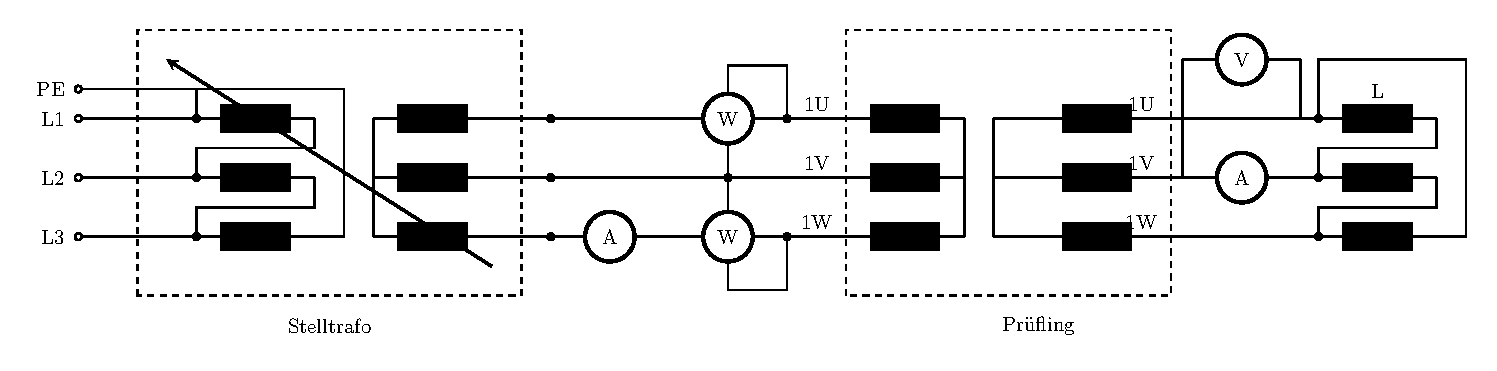
\includegraphics[width=0.95\textwidth]{fig/inductiv_mess.pdf}
    \caption{Messschaltung }
    \label{fig:my_label}
\end{figure}

\begin{figure}[H]
\centering
	\begin{tikzpicture}
		\begin{axis}[
				/pgf/number format/.cd,
				use comma,
				1000 sep={},
				xlabel=$I_{2L} $ (A),
				ylabel={$ U_{2L} \; (\si{\volt})$},
			]
			%The mockup experiment data is stored in a csv file, and imported here.
			\addplot table [x=I_2L (A), y=U_2L, col sep=comma] {data/induk.csv};
			%\addplot table [x=I_2kl, y=I_2kl, col sep=comma] {data/ohmsche_belastung.csv};
		\end{axis}
	\end{tikzpicture}
\end{figure}